Some definitions and results that are used throughout the text are given in this chapter.

\section{Disk}

A circle (or circumference) is a set of points in $\R^2$ that have constant euclidean distance, also known as radius, to another point, also referred to as the center of the circle. A unit circle is a circle with radius equal to $1$.
A disk is the set of points of a circle plus its interior

\begin{definicao}
Let $q \in \R^2$, a unit disk centered at $q$ is the set of points that satisfy \autoref{equation:disk_eq}

\begin{equation}\label{equation:disk_eq}
    (x-q_x)^2 + (y-q_y)^2 \le 1
\end{equation}
\end{definicao}


\section{Ellipse}
An ellipse is the set of all points which have the sum of the distances to two focal points constant. Several equations and parametrizations can be derived from this definition, here they are gonna separated in two cases, the axis parallel and the non axis parallel case.

The axis of an ellipse is the line that passes through its two focal points. An ellipse is considered axis parallel, if its axis is parallel to the $x$-axis.

\subsection{Axis parallel}

An axis parallel ellipse centered at $(0,0)$ can be described by two shape parameters: $a \in \R_{>0}$ the semi-major, $b \in \R_{>0}$ the semi-minor. Its equation is given by \ref{equation:pellipse}

\begin{equation}\label{equation:pellipse}
    \dfrac{x^2}{a^2} + \dfrac{y^2}{b^2} = 1
\end{equation}

\begin{figure}[H]
\centering

    \caption{View of the ellipses parameters}
    

%\tikzset{every picture/.style={line width=0.75pt}} %set default line width to 0.75pt        

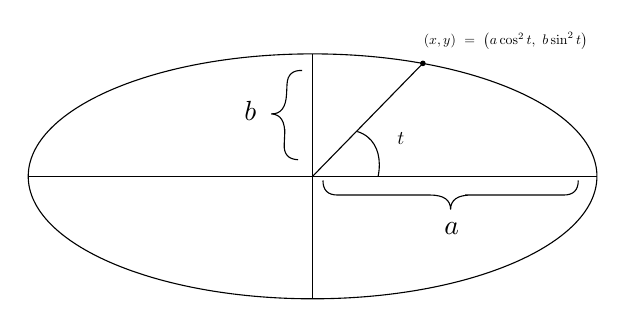
\begin{tikzpicture}[x=0.75pt,y=0.75pt,yscale=-1,xscale=1]
%uncomment if require: \path (0,300); %set diagram left start at 0, and has height of 300

%Shape: Ellipse [id:dp1559950964552308] 
\draw   (100,180) .. controls (100,147.42) and (161.34,121) .. (237,121) .. controls (312.66,121) and (374,147.42) .. (374,180) .. controls (374,212.58) and (312.66,239) .. (237,239) .. controls (161.34,239) and (100,212.58) .. (100,180) -- cycle ;
%Straight Lines [id:da3716259356733107] 
\draw    (100,180) -- (374,180) ;


%Straight Lines [id:da9880464900454329] 
\draw    (237,121) -- (237,239) ;


%Shape: Brace [id:dp3973633345998604] 
\draw   (242,182) .. controls (242,186.67) and (244.33,189) .. (249,189) -- (293.5,189) .. controls (300.17,189) and (303.5,191.33) .. (303.5,196) .. controls (303.5,191.33) and (306.83,189) .. (313.5,189)(310.5,189) -- (358,189) .. controls (362.67,189) and (365,186.67) .. (365,182) ;
%Shape: Brace [id:dp94498526835576] 
\draw   (232,129) .. controls (227.34,128.79) and (224.9,131.01) .. (224.68,135.67) -- (224.47,140.23) .. controls (224.16,146.89) and (221.68,150.11) .. (217.01,149.9) .. controls (221.68,150.11) and (223.85,153.55) .. (223.54,160.21)(223.68,157.21) -- (223.33,164.68) .. controls (223.12,169.35) and (225.34,171.79) .. (230,172) ;
%Shape: Arc [id:dp3154280429415799] 
\draw  [draw opacity=0] (258.54,158.43) .. controls (260.37,158.96) and (262.06,159.82) .. (263.54,161.03) .. controls (268.5,165.07) and (270.12,172.1) .. (268.62,179.79) -- (244.51,184.38) -- cycle ; \draw   (258.54,158.43) .. controls (260.37,158.96) and (262.06,159.82) .. (263.54,161.03) .. controls (268.5,165.07) and (270.12,172.1) .. (268.62,179.79) ;
%Shape: Circle [id:dp8908034615999807] 
\draw  [fill={rgb, 255:red, 0; green, 0; blue, 0 }  ,fill opacity=1 ] (289.08,125.57) .. controls (289.08,124.98) and (289.56,124.51) .. (290.14,124.51) .. controls (290.73,124.51) and (291.21,124.98) .. (291.21,125.57) .. controls (291.21,126.16) and (290.73,126.64) .. (290.14,126.64) .. controls (289.56,126.64) and (289.08,126.16) .. (289.08,125.57) -- cycle ;
%Straight Lines [id:da6323920079482996] 
\draw    (290.14,125.57) -- (237,180) ;



% Text Node
\draw (304,205) node   {$a$};
% Text Node
\draw (207,148.33) node   {$b$};
% Text Node
\draw (330,114.67) node [scale=0.5]  {$( x,y) \ =\ \left( a\cos^{2} t,\ b\sin^{2} t\right)$};
% Text Node
\draw (279.6,162) node [scale=0.7]  {$t$};


\end{tikzpicture}

    \fautor
    \label{fig:3ellipses_intersect}
\end{figure}


\begin{definicao}
An axis-parallel ellipse centered at $(c_x, c_y) \in \R^2$, with shape parameters $(a,b) \in \R^2_{>0}$ is said to cover a point $p=(p_x,p_y)$ if the \autoref{equation:cover_ellipse} is satisfied.

\begin{equation}\label{equation:cover_ellipse}
    \dfrac{(p_x-c_x)^2}{a^2} + \dfrac{(p_y-c_y)^2}{b^2} \le 1
\end{equation}
\end{definicao}

In other words, a point is considered covered by an ellipse if it lies inside, or in the border of the region determined by it.

No equivalent disk-circle wording exists for ellipses, this could be a source of ambiguity in the text, that is why a note for the reader was judged to be necessary. Throughout this work an ellipse will represent the set of points that satisfy \autoref{equation:pellipse}. In some places, though, with prior clarification, we will denote as an ellipse, the set of points that satisfy \autoref{equation:cover_ellipse}. For example, when we define $\Pp \cap E$ as the set of points in $\Pp$ that are covered by $E$, we are implicityly calling $E$ the set of points that satisfy \autoref{equation:cover_ellipse}.